\section{Introducción}

{
\setbeamercolor{background canvas}{bg=beamer@blendedblue!30}
\begin{frame}
  % frame contents here
    \centering
  \Huge
  Introducción
\end{frame}
}

% 
\begin{frame}

\frametitle{Sistema Real}
\begin{block}{Sistema Real}
Partículas auto-propulsadas
\end{block}

\begin{alertblock}{Objetivo}
Investigar su auto-organización a partir de su interacción.
\end{alertblock}

\end{frame}

%
\begin{frame}
\frametitle{Modelo de partículas auto-propulsadas}
\begin{columns}[T] % Align columns at the top
    \begin{column}{0.4\textwidth}
      \begin{center}
        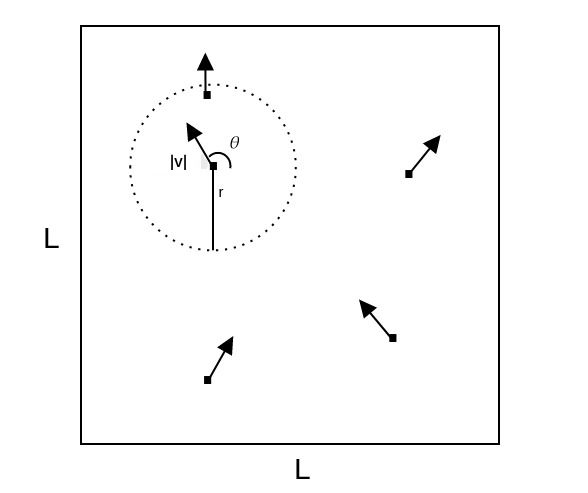
\includegraphics[width=\textwidth]{images/model.jpeg} % Replace with your image file 
      \end{center}
    \end{column}
    \begin{column}{0.6\textwidth}
        \footnotesize Reglas base del modelo:
        \begin{itemize}
            \item Cada partícula se desplaza en cada paso temporal
            \item Velocidad de módulo constante
            \item La dirección es un promedio de direcciones de velocidades vecinas en un radio de interacción "r" \footnote{El cálculo incluye el angulo de la propia partícula}
            \item Se adiciona ruido al cálculo de la dirección promedio    
        \end{itemize}
    \end{column}
\end{columns}
\end{frame}

% Opciones de items 
%
% La dirección se obtiene promediando dentro de un radio de interacción "r" las direcciones de las velocidades de las partículas vecinas.

%
\begin{frame}
\frametitle{Modelo de partículas auto-propulsadas}

Posición de la i-ésima partícula para cada tiempo $t$:
\begin{align}
     \boxed{x_i(t+1) = x_i(t) + v_i(t) \Delta t \text{, } \Delta t = 1}
\end{align}

La dirección de la velocidad se obtiene a partir de la expresión:
\begin{align}
    \boxed{\theta (t+1) = \langle \theta (t) \rangle_r + \Delta \theta}
\end{align}

\begin{alertblock}{$\langle \theta (t) \rangle ~ y ~ \Delta \theta$}
Cálculo del promedio de los ángulos:

\begin{align}
 \langle \theta (t) \rangle_r  = atan2 \left[ \frac{\langle sin(\theta (t)) \rangle_r}{\langle cos(\theta (t)) \rangle_r} \right]
\end{align}

$\Delta \theta$ es el ruido y se obtiene de una distribución unifrome de intervalo $[-\frac{\eta}{2}, \frac{\eta}{2}]$

\end{alertblock}

\end{frame}

